\documentclass[border=10pt]{standalone}

\usepackage{tikz}
\usepackage{tikzsymbols}
\usetikzlibrary{calc,patterns,shapes.geometric}

\def\centerarc[#1](#2)(#3:#4:#5){\draw[#1] ($(#2)+({#5*cos(#3)},{#5*sin(#3)})$) arc (#3:#4:#5);}

\begin{document}
	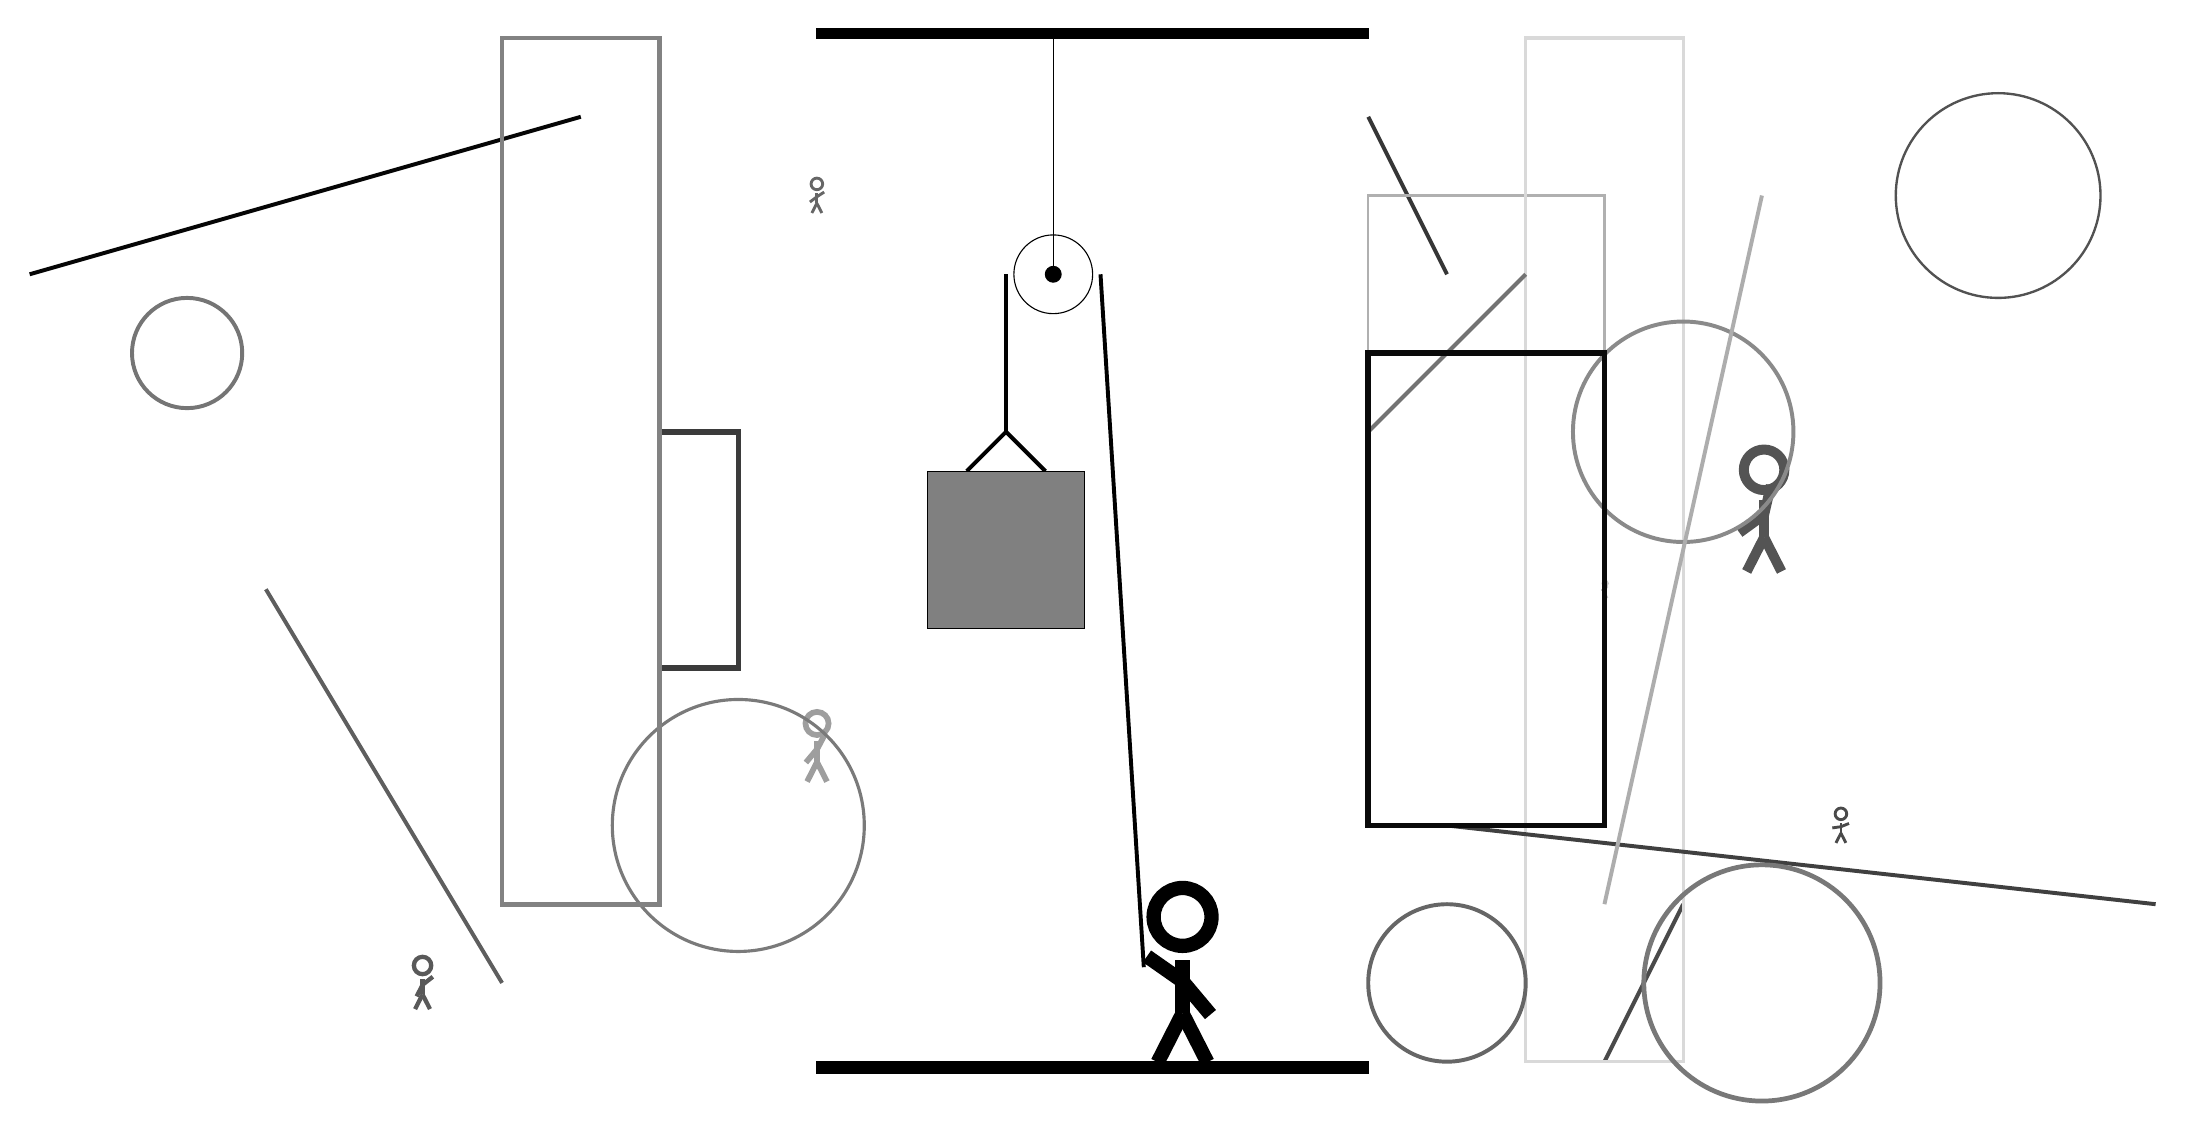
\begin{tikzpicture}
		%%%%% START %%%%%
		
		\draw[fill=black] (-2, 10) rectangle (5, 10.125);
		
		\draw (1, 7) circle (0.5);
		\draw[fill=black] (1, 7) circle (0.1);
		\draw (1, 10) -- (1, 7);
		
		\node[line width=0.7mm, color=black!60] at (-2, 8) {\Strichmaxerl[2][37][33]};
		
		\draw[line width=0.5mm, color=black!98](-5, 9) -- (-12, 7);
		\draw [line width=0.5mm, color=black!54](-10, 6) circle (0.7);
		\draw[line width=0.5mm, color=black!79](6, 7) -- (5, 9);
		\draw[line width=0.3mm, color=black!31] (5, 8) rectangle (8, 6);
		\node[line width=0.6mm, color=black!38] at (-2, 1) {\Strichmaxerl[4][50][62]};
		\draw[line width=0.5mm, color=black!63](-6, -2) -- (-9, 3);
		\draw[line width=0.5mm, color=black!71](9, -1) -- (8, -3);
		\draw[line width=0.4mm, color=black!15] (7, -3) rectangle (9, 10);
		
		\node[line width=0.5mm, color=black!67] at (10, 4) {\Strichmaxerl[7][36][77]};
		\node[line width=0.7mm, color=black!22] at (8, 3) {\Strichmaxerl[1][0][52]};
		\node[line width=0.4mm, color=black!65] at (-7, -2) {\Strichmaxerl[3][63][38]};
		\node[line width=0.3mm, color=black!71] at (11, 0) {\Strichmaxerl[2][8][22]};
		
		\draw [line width=0.5mm, color=black!46](9, 5) circle (1.4);
		\draw [line width=0.5mm, color=black!60](6, -2) circle (1.0);
		\draw[line width=0.5mm, color=black!75](6, 0) -- (15, -1);
		\draw[line width=0.5mm, color=black!55](7, 7) -- (5, 5);
		\draw[line width=0.7mm, color=black!77] (-4, 2) rectangle (-3, 5);
		\draw[line width=0.5mm, color=black!32](10, 8) -- (8, -1);
		\draw [line width=0.3mm, color=black!68](13, 8) circle (1.3);
		\draw [line width=0.4mm, color=black!52](-3, 0) circle (1.6);
		
		\draw[line width=0.7mm, color=black!96] (5, 0) rectangle (8, 6);
		\draw [line width=0.6mm, color=black!53](10, -2) circle (1.5);
		\draw[line width=0.6mm, color=black!49] (-4, -1) rectangle (-6, 10);
		
		\draw[line width=0.5mm] (-0.1, 4.5) -- (0.4, 5.0) -- (0.9, 4.5);
		\draw[fill=black!50] (-0.6, 4.5) rectangle (1.4, 2.5);
		
		\draw[line width=0.5mm] (0.4, 7) -- (0.4, 5.0);
		\centerarc[line width=0.5mm](1, 7)(0:180:0.6);
		\draw[line width=0.5mm](1.6, 7) -- (2.15, -1.8);
		
		\node at (2.6, -1.9) {\Strichmaxerl[10][-35][-50]};
		
		\draw[fill=black] (-2, -3) rectangle (5, -3.15);
		
		%%%%% END %%%%%
	\end{tikzpicture}
\end{document}